\refstepcounter{chapter}
\addcontentsline{toc}{chapter}{Disassembly Instructions}

\setsectiontitle{Main Motor}

\begin{figure}[H]
    \centering
    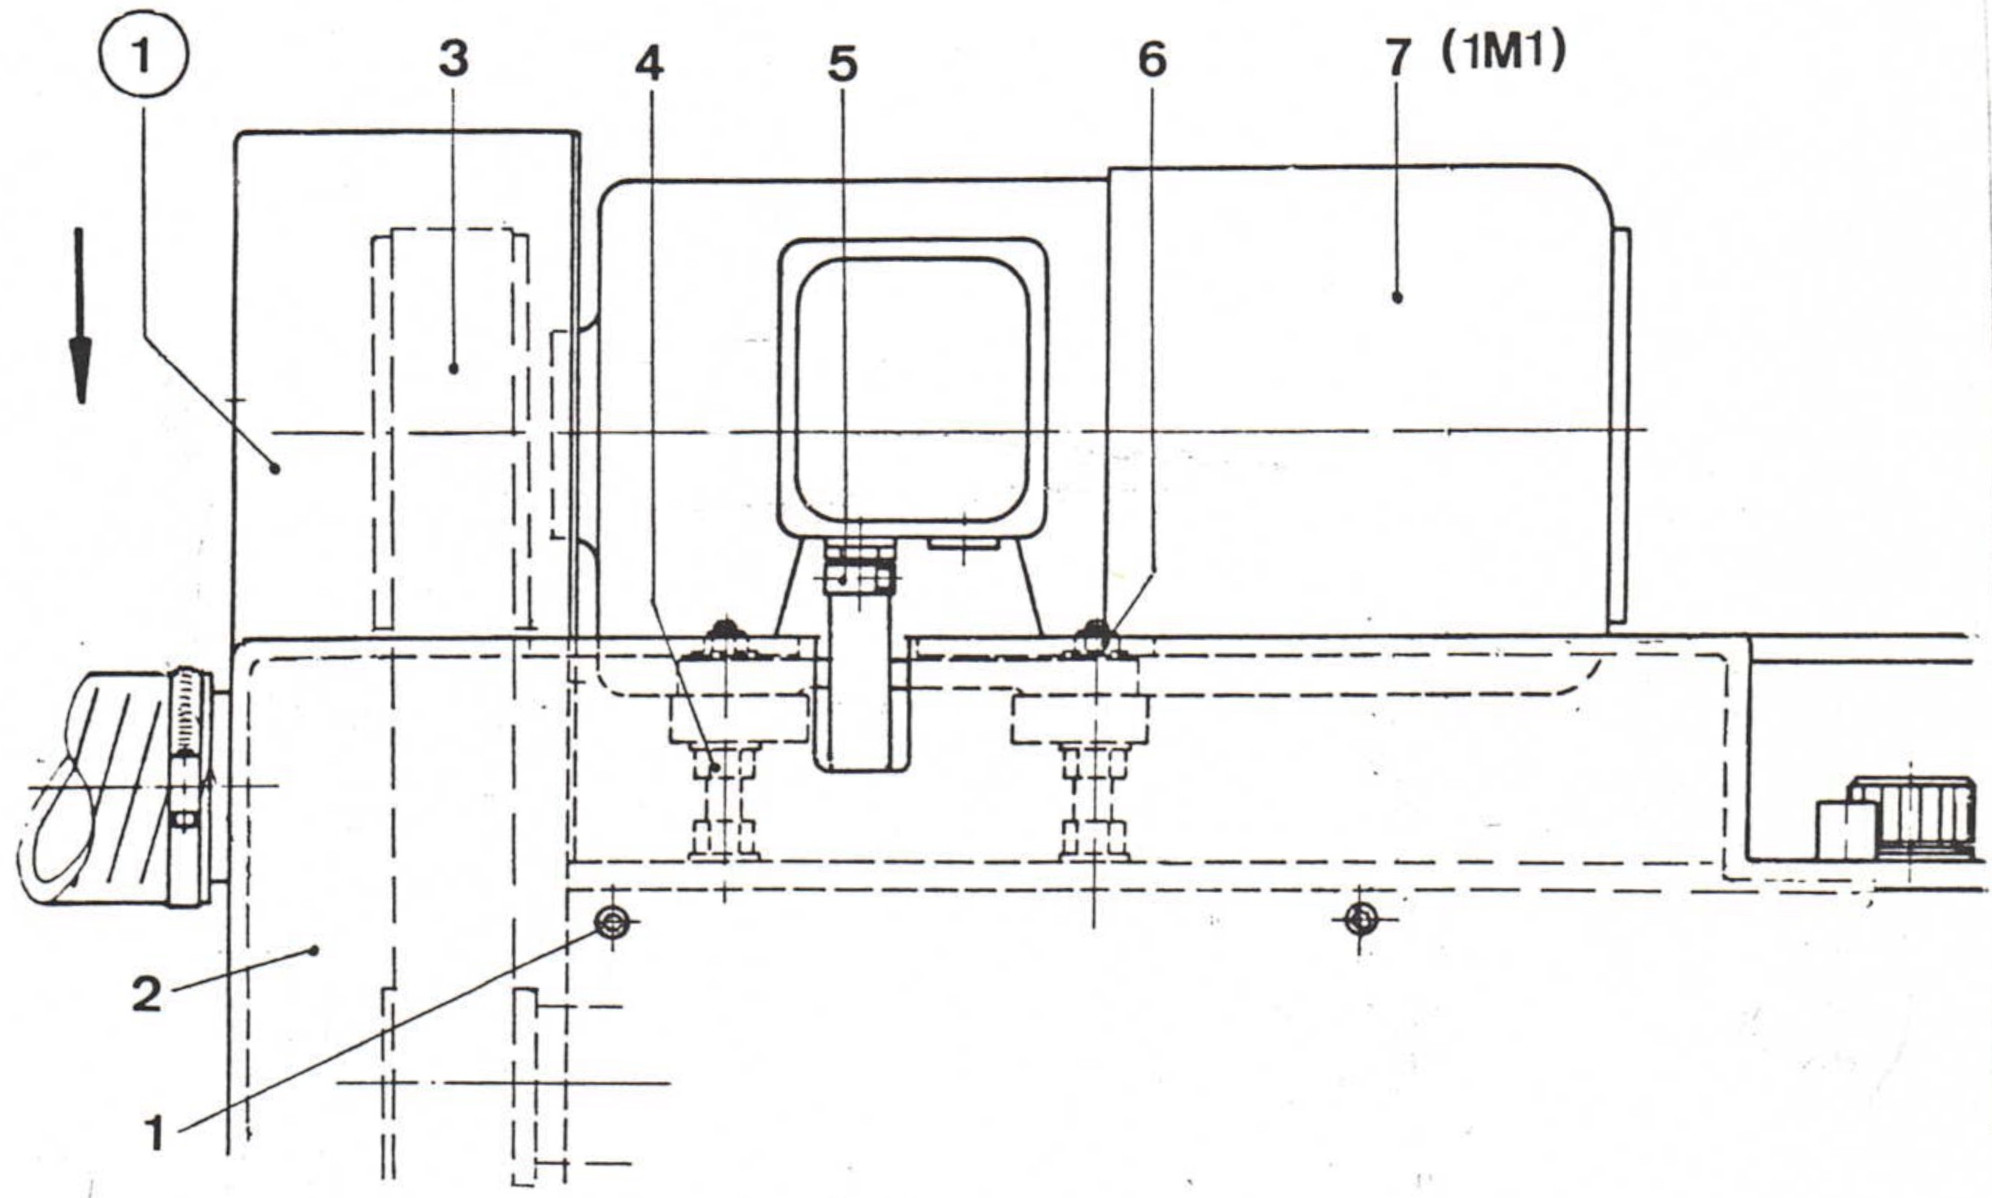
\includegraphics[width=0.85\textwidth]{images/chapter9/main_motor_disassembly.jpg}
    \label{fig:main_motor_disassembly}
\end{figure}

\subsection*{Disassembly}

\begin{itemize}
    \setlength{\itemsep}{0pt} \setlength{\parskip}{0pt}
    \item Switch off the \textbf{main switch Q1} on the control cabinet.
    \item Disconnect the \textbf{connection cable \circled{5}} from the motor \circled{7} (1M1).
    \item Remove the \textbf{screws \circled{1}} and take off the \textbf{cover \circled{2}}.
    \item Remove the \textbf{belt guard \circled{7}} as instructed on page 7.10-1.
    \item Unscrew the \textbf{nuts \circled{6}}.
\end{itemize}

\notebox{WARNING}{%
    The \textbf{lower nuts \circled{4}} must not be adjusted.
}

\begin{itemize}
    \setlength{\itemsep}{0pt} \setlength{\parskip}{0pt}
    \item Tilt the \textbf{motor \circled{7}} in the direction of the arrow and remove the \textbf{belt \circled{3}}.
    \item Lift the \textbf{motor \circled{7}} off the spindle head.
\end{itemize}

\subsection*{Reassembly}

\begin{itemize}
    \setlength{\itemsep}{0pt} \setlength{\parskip}{0pt}
    \item Reassembly is performed in reverse order.
    \item The \textbf{belt pulleys must be aligned}. \footnotemark[1]
    \item The \textbf{motor shaft must be exactly parallel} to the spindle head. \footnotemark[1]
\end{itemize}

\footnotetext[1]{For assembly and maintenance of the V-ribbed belt, see page 7.34-1.}

\setsectiontitle{Feed Drive Motor Replacement}

\setcounter{section}{8}

\subsection*{X-Axis}

\begin{itemize}
    \setlength{\itemsep}{0pt} \setlength{\parskip}{0pt}
    \item Switch off the \textbf{main switch Q1} on the control cabinet.  
          To prevent accidental reactivation, the main fuses can be removed from the control cabinet.
    \item Disconnect the \textbf{connector} from the \textbf{motor \circled{3}}.
    \item Loosen the \textbf{socket head screws \circled{1}}.
    \item Tilt the \textbf{motor \circled{3}} toward the lead screw until the \textbf{timing belt \circled{5}} can be removed from the \textbf{motor shaft \circled{2}}.
    \item Remove the \textbf{motor \circled{3}}.
    \item Insert the \textbf{new motor \circled{3}}, place the \textbf{timing belt \circled{5}} onto the \textbf{motor shaft \circled{2}},  
          and shift the motor until the timing belt is moderately tensioned.
    \item Tighten the \textbf{socket head screws \circled{1}}.
    \item Reconnect the \textbf{connector} to the \textbf{motor \circled{3}}.
\end{itemize}

\begin{figure}[H]
    \centering
    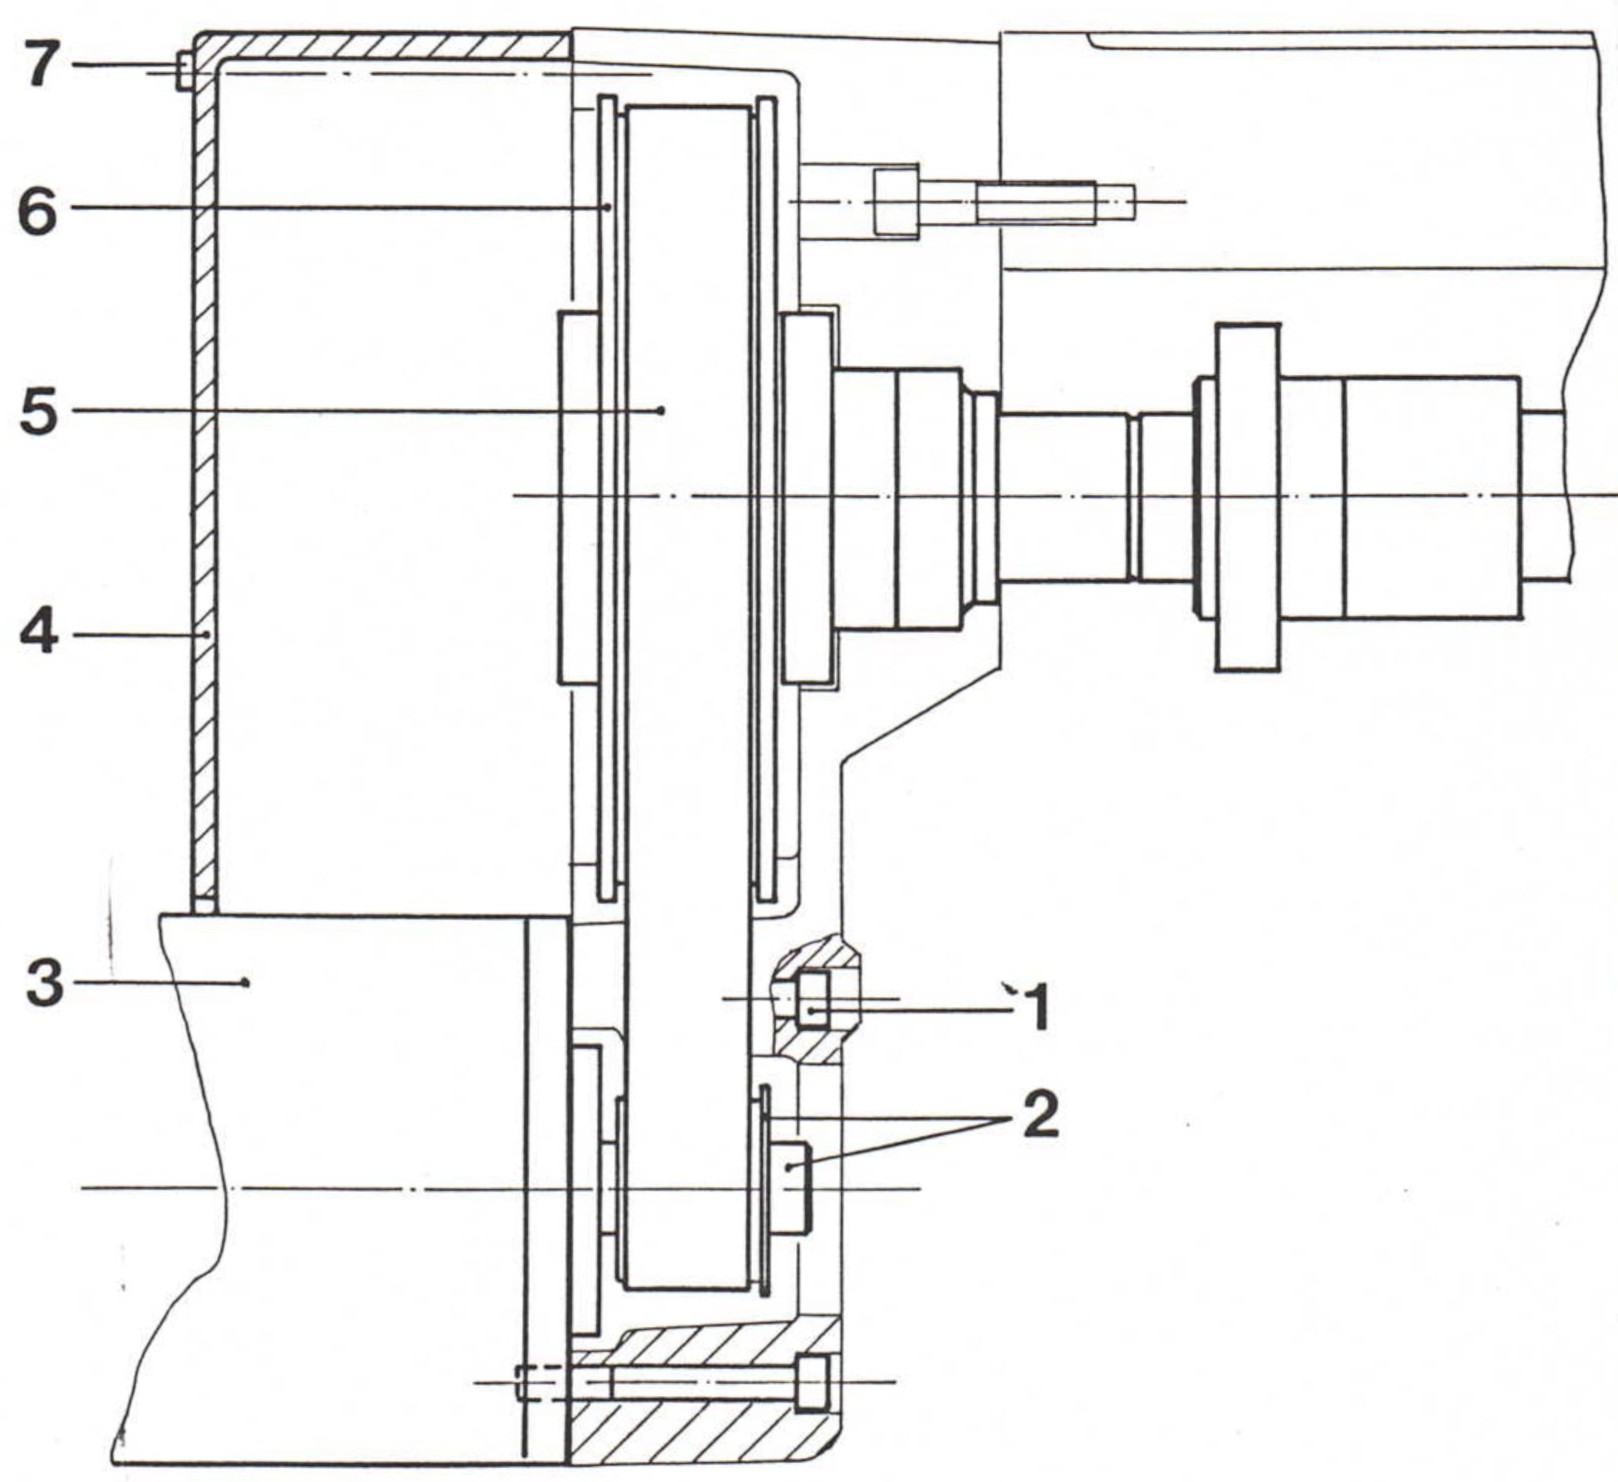
\includegraphics[width=0.85\textwidth]{images/chapter9/feed_drive_motor_x_axis.jpg}
    \label{fig:feed_drive_motor_x_axis}
\end{figure}

\newpage

\subsection*{Y-Axis}

\begin{figure}[H]
    \centering
    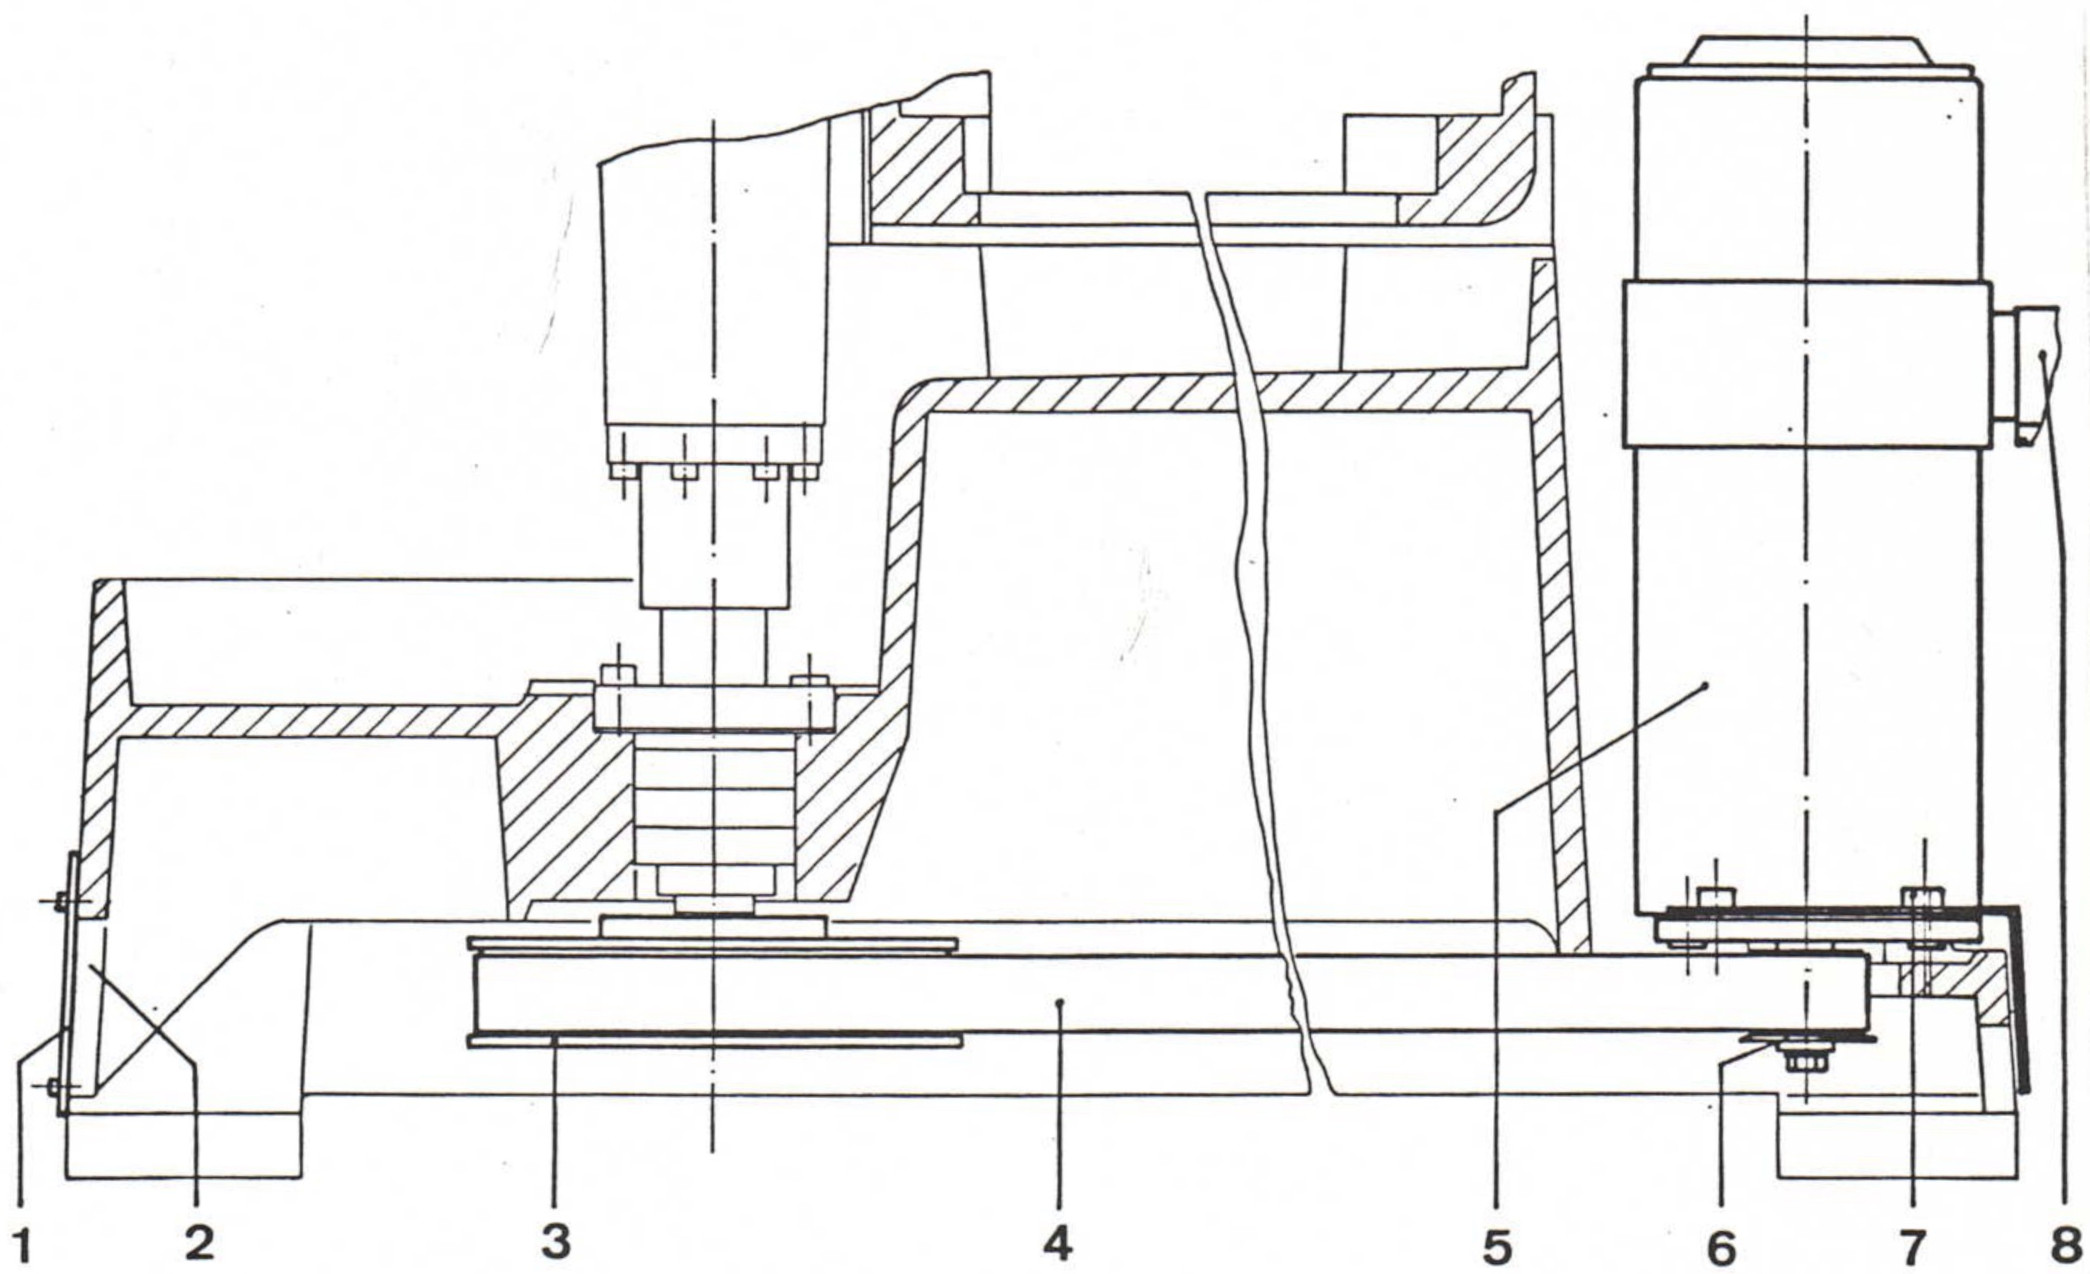
\includegraphics[width=0.85\textwidth]{images/chapter9/feed_drive_motor_y_axis.jpg}
    \label{fig:feed_drive_motor_y_axis}
\end{figure}

\begin{itemize}
    \setlength{\itemsep}{0pt} \setlength{\parskip}{0pt}
    \item Move the \textbf{cross slide} to the upper end position and support it.
    \item Switch off the \textbf{main switch Q1} on the control cabinet.  
          To prevent accidental reactivation, the main fuses can be removed from the control cabinet.
    \item Remove the \textbf{machine covers \circled{2}} (see page 7.10-1).
    \item Disconnect the \textbf{connector \circled{8}} from the \textbf{motor \circled{5}}.
    \item Remove the \textbf{screws \circled{7}}, then tilt and carefully lift out the \textbf{motor \circled{5}}.
    \item Carefully insert the \textbf{new motor \circled{5}}, ensuring the \textbf{timing belt \circled{4}} is positioned onto the \textbf{timing pulley \circled{6}}.
    \item Adjust the belt tension by shifting the \textbf{motor \circled{5}}, then tighten the \textbf{screws \circled{7}}.
    \item Reconnect the \textbf{connector \circled{8}} to the \textbf{motor \circled{5}} and reinstall the \textbf{machine covers \circled{2}}.
\end{itemize}

\newpage

\subsection*{Z-Axis}

\begin{itemize}
    \setlength{\itemsep}{0pt} \setlength{\parskip}{0pt}
    \item Remove the \textbf{machine covers \circled{1}, \circled{2}, and \circled{3}} (see page 7.10-1).
    \item Move the \textbf{spindle head} to \textbf{Z 250}.
    \item Switch off the \textbf{main switch Q1} on the control cabinet.  
          To prevent accidental reactivation, the main fuses can be removed from the control cabinet.
    \item Disconnect the \textbf{connector \circled{6}} from the \textbf{motor \circled{5}}.
    \item Loosen the \textbf{socket head screws \circled{4}}.
    \item Tilt the \textbf{motor \circled{5}} to release the \textbf{timing belt \circled{2}} from the \textbf{motor shaft \circled{3}}.
    \item Remove the \textbf{motor \circled{5}}.
    \item Install the \textbf{new motor}, ensuring the \textbf{timing belt \circled{2}} is properly placed onto the \textbf{motor shaft \circled{3}}.
    \item Partially tighten the \textbf{socket head screws \circled{4}},  
          check the belt tension, then fully secure them.
    \item Reconnect the \textbf{connector \circled{6}}, then reinstall the \textbf{machine covers \circled{1}, \circled{2}, and \circled{3}}.
\end{itemize}

\begin{figure}[H]
    \centering
    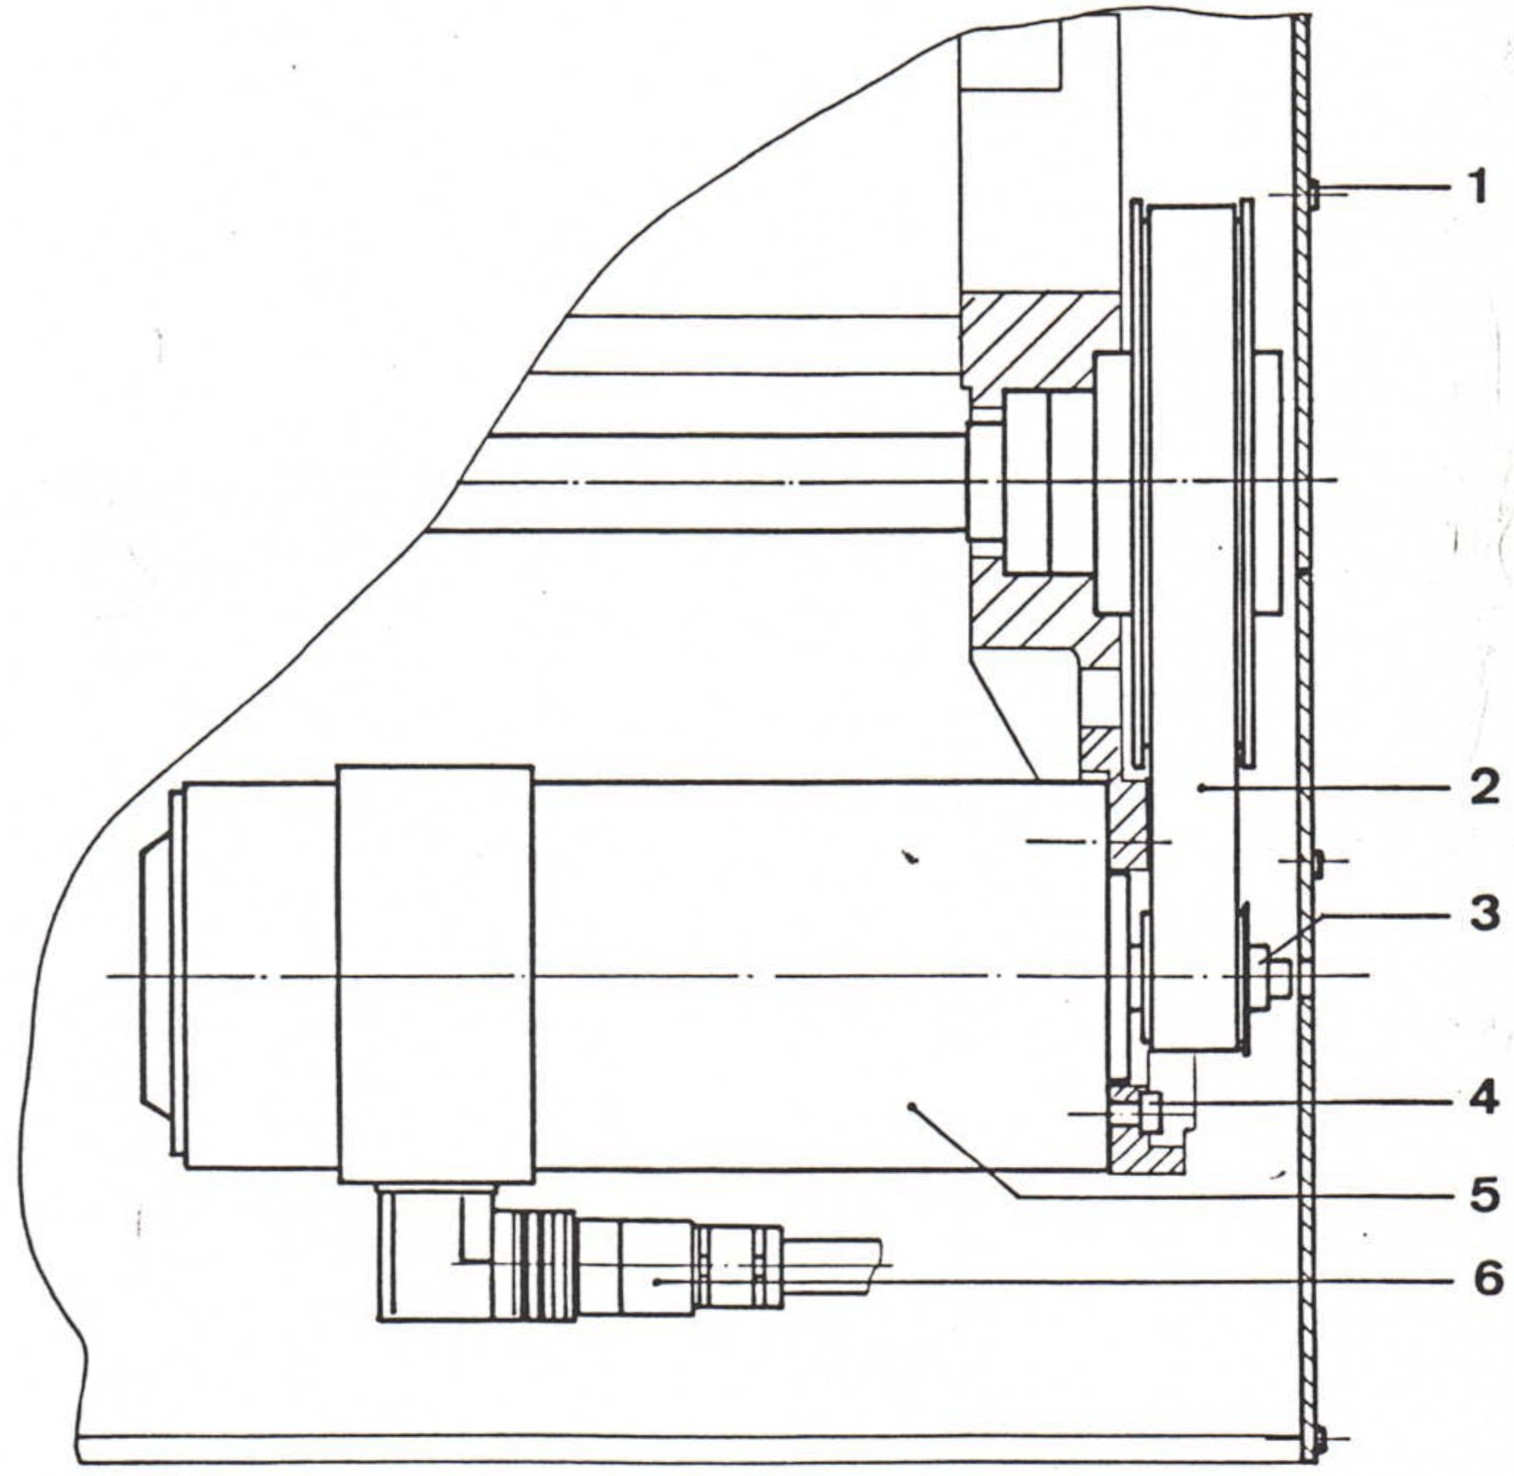
\includegraphics[width=0.85\textwidth]{images/chapter9/feed_drive_motor_z_axis.jpg}
    \label{fig:feed_drive_motor_z_axis}
\end{figure}
